% Created 2026-03-26 Thu 18:45
% Intended LaTeX compiler: pdflatex
\documentclass[presentation, aspectratio=169]{beamer}
\usepackage[utf8]{inputenc}
\usepackage[T1]{fontenc}
\usepackage{graphicx}
\usepackage{grffile}
\usepackage{longtable}
\usepackage{wrapfig}
\usepackage{rotating}
\usepackage[normalem]{ulem}
\usepackage{amsmath}
\usepackage{textcomp}
\usepackage{amssymb}
\usepackage{capt-of}
\usepackage{hyperref}
\mode<beamer>{\usetheme{Madrid}}
\usepackage{tikz}
\usetikzlibrary{shapes,backgrounds,positioning,arrows.meta}
\mode<beamer>{\usetheme{Madrid}}
\usepackage{minted}
\usemintedstyle{emacs}
\DeclareMathOperator*{\maxim}{maximize}
\DeclareMathOperator*{\minim}{minimize}
\usetheme{default}
\usecolortheme{default}
\usefonttheme{default}
\author{João Pedro PEDROSO|DIONÍSIO}
\date{\alert{\alert{2026 APDIO Workshop: Optimization Software \& Practice\newline University of Minho, 27-MAR-2026}}}
\title{Modeling languages: alpha and omega}
\institute[FCUP]{Faculty of Sciences, University of Porto}
\titlegraphic{
\includegraphics[height=1.5cm]{FIGS/cmup-info.png}}
\hypersetup{
 pdfauthor={João Pedro PEDROSO|DIONÍSIO},
 pdftitle={Modeling languages: alpha and omega},
 pdfkeywords={},
 pdfsubject={},
 pdfcreator={Emacs 30.2 (Org mode 9.4.6)}, 
 pdflang={American}}
\begin{document}

\maketitle
\begin{frame}{Outline}
\tableofcontents
\end{frame}


\section{The "Alpha" of Optimization}
\label{sec:org1eb9410}

\begin{frame}[label={sec:org1a3dd7c}]{Background}
\begin{itemize}
\item We have a system of linear inequalities.
\item How can we find a feasible solution?
\item In particular, can we choose a feasible solution that optimizes some (linear) criterion?
\begin{itemize}
\item \emph{note: that amounts to optimizing an expression, which can be assigned to a variable.}
\end{itemize}
\end{itemize}
\end{frame}


\begin{frame}[label={sec:orgff52cfc}]{The Pre-History: Joseph Fourier (1826)}
\begin{block}{The Concept of Projection}
Before the Simplex Method: Fourier devised a method for solving systems of linear inequalities:
\begin{itemize}
\item \alert{\alert{Method}}: Fourier–Motzkin Elimination.
\item \alert{\alert{Goal}}: Determining the feasibility of undetermined systems.
\item \alert{\alert{Insight}}: Optimization (min-max) is equivalent to solving inequalities.
\end{itemize}
\end{block}
\end{frame}


\begin{frame}[label={sec:org3c2cfbc}]{Comparing "Projecting" vs. "Walking"}
\begin{itemize}
\item Fourier (1826):
\begin{itemize}
\item Project the \(n\text{-dimensional}\) feasible region onto lower dimensions.
\end{itemize}
\item Dantzig (1947):
\begin{itemize}
\item \emph{\alert{Simplex Method:}} Move between vertices of the \(n\text{-dimensional}\) region.
\end{itemize}
\end{itemize}
\end{frame}


\begin{frame}[label={sec:org07aaf92}]{Visualizing the Two Approaches}
\begin{block}{Vertex Walk vs. Projection}
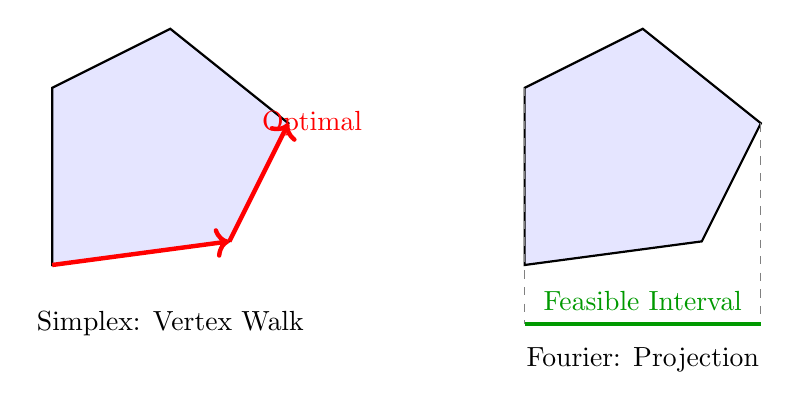
\begin{tikzpicture}[scale=1.5]
  % Left side: Simplex (Vertex Walk)
  \begin{scope}[xshift=-2cm]
    \draw[thick, fill=blue!10] (0,0) -- (1.5,0.2) -- (2,1.2) -- (1,2) -- (0,1.5) -- cycle;
    \draw[->, ultra thick, red] (0,0) -- (1.5,0.2);
    \draw[->, ultra thick, red] (1.5,0.2) -- (2,1.2);
    \node at (1, -0.5) {Simplex: Vertex Walk};
    \node[red] at (2.2, 1.2) {Optimal};
  \end{scope}

  % Right side: Fourier-Motzkin (Projection)
  \begin{scope}[xshift=2cm]
    \draw[thick, fill=blue!10] (0,0) -- (1.5,0.2) -- (2,1.2) -- (1,2) -- (0,1.5) -- cycle;
    \draw[dashed, gray] (0,1.5) -- (0,-0.5);
    \draw[dashed, gray] (2,1.2) -- (2,-0.5);
    \draw[ultra thick, green!60!black] (0,-0.5) -- (2,-0.5);
    \node at (1, -0.8) {Fourier: Projection};
    \node[green!60!black] at (1, -0.3) {Feasible Interval};
  \end{scope}
\end{tikzpicture}
\end{block}
\end{frame}


\begin{frame}[label={sec:orgc6ecd5b}]{Fourier's Method "Explodes"}
\begin{itemize}
\item \alert{Fourier-Motzkin}: Each variable elimination creates a new set of inequalities.
\begin{itemize}
\item If we have \(m\) inequalities, eliminating one variable can result in up to \((m/2)^2\) new ones.
\item Impractical for the next example (Stigler's 77 variables).
\item Theoretically important (e.g., for proving the Farkas Lemma).
\end{itemize}
\item \alert{Simplex}: Complexity depends on the number of \alert{vertices} (usually efficient).
\end{itemize}

\begin{block}{Historical Note}
Dantzig noted that had he known Fourier–Motzkin Elimination he might have been discouraged by the perceived complexity of inequality systems.
\end{block}
\end{frame}


\begin{frame}[label={sec:orgd0b4527}]{The Stigler Diet Problem (1947)}
\begin{block}{A Problem in the "Alpha" Era}
George Stigler (1945) sought the minimum cost to feed a 154lb man.
\begin{itemize}
\item \alert{\alert{Goal}}: Minimize daily cost of food.
\item \alert{\alert{Scale}}: 77 candidate foods, 9 nutritional constraints.
\end{itemize}
\end{block}

\begin{block}{Mathematical Formulation}
\begin{itemize}
\item Minimize \(Z = \sum_{j=1}^{77} c_j x_j\)

\item Subject to: \(\sum_{j=1}^{77} a_{ij} x_j \ge b_i \quad \forall i \in \{1, \dots, 9\}\), \qquad
\(x_j \ge 0 \quad \forall j \in \{1, \dots, 77\}\)

\item Where:
\begin{itemize}
\item \(c_j\): Cost of food \(j\)
\item \(a_{ij}\): Amount of nutrient \(i\) in food \(j\)
\item \(b_i\): recommended daily allowance for nutrient \(i\) \\
calories, protein, calcium, iron, vitamin A, B1, B2, niacin, vitamin C
\end{itemize}
\end{itemize}
\end{block}
\end{frame}


\begin{frame}[label={sec:org476f27a}]{The Human "Computer": Jack Laderman's Achievement}
\begin{block}{Before Machines}
In 1947, the "Simplex Method" was brand new (Dantzig). There was no "software."
\begin{itemize}
\item \alert{\alert{Team}}: 9 human clerks at the National Bureau of Standards.
\item \alert{\alert{Hardware}}: Hand-operated desk calculators
\item \alert{\alert{Effort}}: \alert{\alert{120 man-days}} of computation.
\end{itemize}
\end{block}

\begin{block}{Results}
\begin{itemize}
\item Stigler’s heuristic guess: \$39.93/year (1939 prices).
\item Laderman’s Simplex solution: \$39.69/year.
\item \alert{Fun Fact}: The "optimal" diet consisted mostly of wheat flour, evaporated milk, cabbage, spinach, and navy beans. Stigler called it the "human dog biscuit."
\end{itemize}
\end{block}
\end{frame}


\begin{frame}[label={sec:orga720ed8}]{First Machine Implementations: SEAC and IBM 701}
\begin{block}{SEAC (1951) - The First Electronic Solver}
\begin{itemize}
\item \alert{\alert{Machine}}: Standards Eastern Automatic Computer (National Bureau of Standards).
\item \alert{\alert{Implementation}}: First general-purpose Simplex code for a stored-program computer.
\item \alert{\alert{Language}}: \alert{\alert{Machine Code / Binary}} (no high-level languages like Fortran existed yet).
\item \alert{\alert{Scale}}: Solved a \(48 \times 71\) Air Force model in minutes.
\end{itemize}
\end{block}

\begin{block}{IBM 701 (1954) - The First "Commercial" Code}
\begin{itemize}
\item Developed at RAND Corporation.
\item Language: \alert{\alert{Assembly}} (highly optimized for the 701's architecture).
\item Could handle \textasciitilde{}100 constraints
\begin{itemize}
\item moved LP from research to the oil industry (refining/blending).
\end{itemize}
\item Beginning of \alert{\alert{Matrix Generators}}
\begin{itemize}
\item (tedious) precursors to the modeling languages we use today.
\end{itemize}
\end{itemize}
\end{block}
\end{frame}


\begin{frame}[label={sec:orgfffe272},fragile]{Before Modeling Languages: Physical Data Entry}
 \begin{block}{The Punched Card Era (1950s)}
In the "Alpha" phase, there was no \texttt{model.lp} or \texttt{model.py}. 

Data was physical.

\begin{itemize}
\item \alert{\alert{Storage}}: IBM 80-column punched cards.
\item \alert{\alert{Method}}: One non-zero coefficient per card.
\item \alert{\alert{Hardware}}: IBM 026 Keypunch and 056 Verifier.
\end{itemize}


\begin{center}
\begin{center}
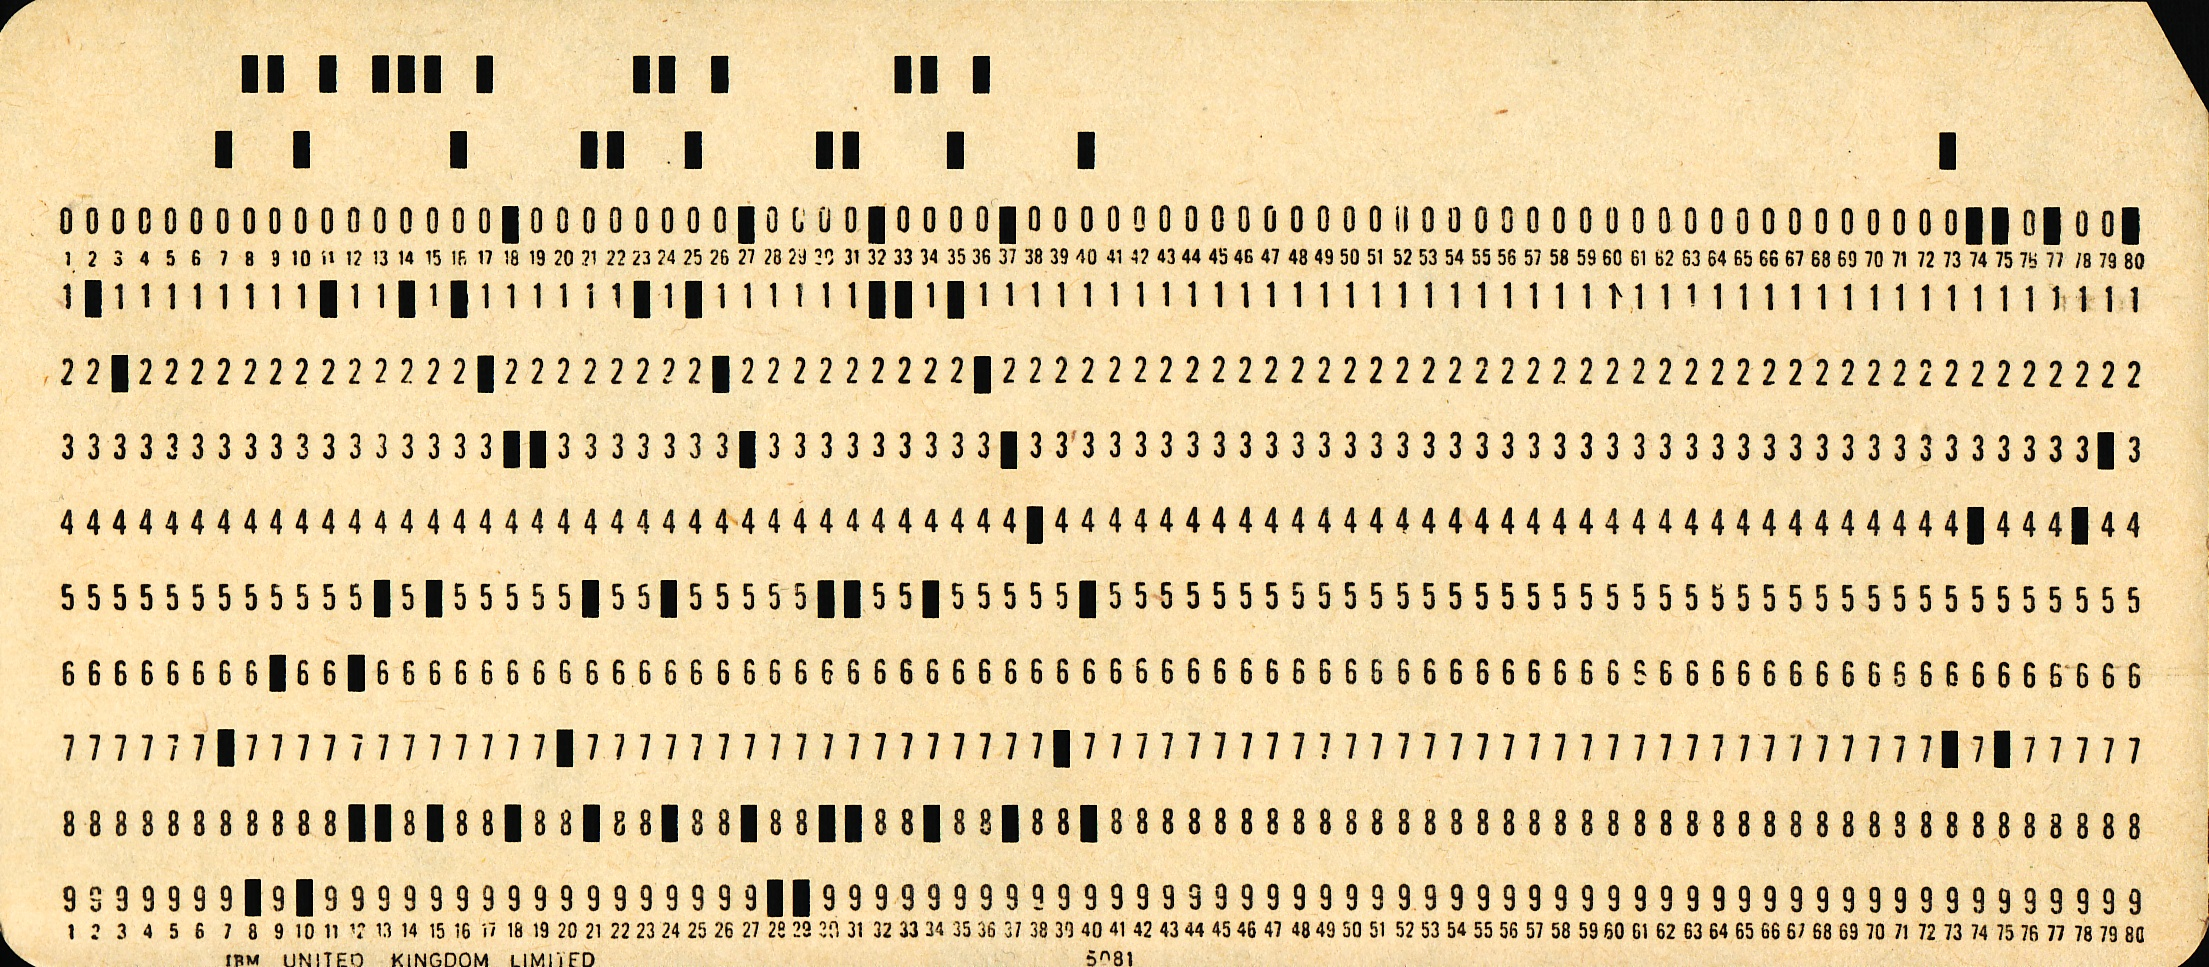
\includegraphics[angle=0,width=.6\textwidth]{FIGS/Used_Punchcard.jpg}
\end{center}
\end{center}
\end{block}
\end{frame}


\begin{frame}[label={sec:orgc43dcf6}]{Before Modeling Languages: Workflow}
\begin{enumerate}
\item \alert{\alert{Mathematical Model}}: written on paper.
\item \alert{\alert{Matrix Tabulation}}: coefficients mapped to row/column indices.
\item \alert{\alert{Keypunching}}: manual transcription to cards.
\item \alert{\alert{Verification}}: mechanical "double-checking" of holes.
\end{enumerate}

\begin{block}{Technical Bottleneck}
\begin{itemize}
\item A typo in one card meant the Simplex algorithm would diverge or find a wrong solution.
\item There was no "algebraic" check, only a mechanical one.
\item \alert{\alert{Transition}}: creation of \alert{Matrix Generators} in the 1960s.
\end{itemize}
\end{block}
\end{frame}


\begin{frame}[label={sec:org2a8741a}]{The "Middle Ages": Matrix Generators}
\begin{block}{The "Logic" of 1965}
\begin{itemize}
\item Instead of writing math, we wrote code to print strings and formatted numbers.
\begin{itemize}
\item specialized "printing" programs usually written in FORTRAN.
\end{itemize}
\item Any mistake in the code makes the MPS file unreadable/wrong.
\item \alert{\alert{Maintenance}}: To add a nutrient, we must change the `DATA` statements, the `DO` loop limits, and potentially the `FORMAT` strings.
\end{itemize}
\end{block}
\end{frame}


\begin{frame}[label={sec:orgf1b0690},fragile]{The "Middle Ages"}
 A Matrix Generator (Fortran)

{\scriptsize
\begin{verbatim}
C     FORTRAN MATRIX GENERATOR FOR STIGLER DIET
      DATA FOODS/'WHEAT', 'CORNM', 'EVAPM', 'MARGA'/
      DATA NUTRI/'COST ', 'CALOR', 'PROT ', 'CALCI'/
      
      WRITE(6, 100) 'NAME', 'STIGLER'
      WRITE(6, 110) 'ROWS'
      WRITE(6, 120) ' N ', 'COST'
      DO 10 I=2, 5
   10 WRITE(6, 120) ' G ', NUTRI(I)
   
      WRITE(6, 110) 'COLUMNS'
      DO 20 J=1, 77
C       INNER LOOP FETCHES DATA FROM ARRAYS AND FORMATS FOR MPS
        WRITE(6, 130) FOODS(J), 'COST', COST(J), 'CALOR', CAL(J)
   20 CONTINUE
   
  100 FORMAT(A4, 10X, A8)
  110 FORMAT(A)
  120 FORMAT(A3, 2X, A8)
  130 FORMAT(4X, A8, 2X, A8, F12.4, 2X, A8, F12.4)
\end{verbatim}
}
\end{frame}


\begin{frame}[label={sec:orge420a95},fragile]{The MPS Format (The Lingua Franca)}
 Standardized by IBM in 1965, it remains the "Assembly Language" of LP.
\begin{itemize}
\item \alert{\alert{Rigid Structure}}: 80-column fixed-field layout (inherited from punched cards).
\item \alert{\alert{Sections}}: \texttt{NAME}, \texttt{ROWS}, \texttt{COLUMNS}, \texttt{RHS}, \texttt{BOUNDS}.
\item \alert{\alert{Persistence}}: Every modern solver (Gurobi, CPLEX, HiGHS) still reads .mps files.
\end{itemize}

\begin{block}{MPS Paradox}
\begin{itemize}
\item Highly efficient for computers to parse.
\item Nearly impossible for humans to debug.
\item This "Readability Gap" is what eventually forced the creation of AMLs.
\end{itemize}
\end{block}
\end{frame}


\begin{frame}[label={sec:orgca066b1},fragile]{MPS Format}
 Example: Stigler Diet in 80 Columns

{\scriptsize
\begin{verbatim}
NAME          STIGLER
ROWS
 N  COST
 G  CALORIES
 G  PROTEIN
 G  CALCIUM
COLUMNS
    WHEAT     COST            0.036     CALORIES       3.3
    WHEAT     PROTEIN         13.3      CALCIUM        0.9
    CORNMEAL  COST            0.018     CALORIES       3.0
    CORNMEAL  PROTEIN         10.0      CALCIUM        2.0
RHS
    RHS1      CALORIES        3.0       PROTEIN        70.0
    RHS1      CALCALCIUM      0.8
ENDATA
\end{verbatim}
}
\end{frame}


\begin{frame}[label={sec:orgb1dfb46},fragile]{The Representation Gap}
 \begin{block}{From Human Thought to Solver Input}
\begin{itemize}
\item Before AMLs (like AMPL or JuMP), there was a "lost in translation" phase.
\begin{itemize}
\item To a mathematician, the model is a set of summations.
\item To the computer, the model is a flat list of entries.
\end{itemize}
\end{itemize}
\end{block}

\begin{block}{Comparison: The Stigler Diet Problem}
\begin{center}
\begin{tabular}{|l|p{7cm}|l|}
\hline
Format & Representation of \(\sum a_{ij}x_j \ge b_i\) & Readability\\
\hline
\alert{\alert{Matrix Generator}} & \texttt{FOR I=1 TO 9: WRITE(6,10) ROW(I), RHS(I)} & Zero\\
\alert{\alert{MPS (Machine)}} & \texttt{COL001    NUTRIENT01  0.0034} & \\
\alert{\alert{Algebraic}} & \(\sum_{j \in J} a_{ij} x_j \ge b_i, \quad \forall i \in I\) & High\\
\hline
\end{tabular}
\end{center}
\end{block}
\end{frame}


\begin{frame}[label={sec:org9c2896b},fragile]{MPS: "Technical Debt" of the 1970s}
 \begin{itemize}
\item In MPS, data and logic are fused:
\begin{itemize}
\item data (\(a_{ij}\)) is separate from logic (a sum).
\item if we add one nutrient to the diet problem, we must recalculate and re-punch the entire file.
\end{itemize}
\item Modeling was slow, error-prone, and required "model librarians".
\item Support for linear programming, with limited extensions added:
\begin{itemize}
\item 1965: original MPS, linear programming.
\item 1969: integer variables \(\to\) \texttt{INTORG} and \texttt{INTEND} markers within the \texttt{COLUMNS} section.
\item 1970: limits on the variables \(\to\) \texttt{BOUNDS} section
\item 1976: piecewise linear functions \(\to\) Special Ordered Sets:
\begin{itemize}
\item \texttt{SOS1}: Only one variable in the set can be non-zero.
\item \texttt{SOS2}: At most two variables can be non-zero, and they must be adjacent (used for approximating curves).
\end{itemize}
\item 1980s: \(x^2\) in the objective: \texttt{QCMATRIX} or \texttt{QUADOBJ}
\end{itemize}
\item but format still rather limited\ldots{}
\end{itemize}
\end{frame}



\section{Model taxonomy}
\label{sec:org1d8e2c0}

\begin{frame}[label={sec:orgbaebdf7}]{Model Taxonomy: Choosing the Right Solver}
\begin{block}{The "Linear" Foundation}
\begin{itemize}
\item \alert{Linear Programming (LP)}: Continuous variables, linear constraints and objective.
\begin{itemize}
\item Standard, typically uses simplex or interior point methods.
\end{itemize}
\item \alert{Mixed-Integer Programming (MIP)*}: Adds discrete choices (\(0/1\)).
\begin{itemize}
\item NP-Hard problems, typically solved with Branch-and-Bound.
\end{itemize}
\end{itemize}
\end{block}

\begin{block}{Beyond Linearity}
\begin{itemize}
\item \alert{Nonlinear Programming (NLP)}: Curved surfaces (e.g., chemical blending, power grids).
\begin{itemize}
\item Local vs. Global optima, typically requires gradient-based solvers.
\end{itemize}
\item \alert{Constraint Programming (CP)}: Logic constraints (e.g., "If A is before B, then C cannot be at 4pm").
\begin{itemize}
\item Applications: Logic programming, Scheduling, Routing.
\end{itemize}
\item \alert{Complementarity problems}: "Either \(x=0\) or the constraint is tight."
\begin{itemize}
\item Applications: Game theory, equilibrium models.
\end{itemize}
\end{itemize}
\end{block}
\end{frame}



\section{The "good" modeling language checklist}
\label{sec:org0c0e64f}
\begin{frame}[label={sec:org023bad5},fragile]{The Renaissance: GAMS (1976)}
 \begin{block}{Algebraic Realism}
In GAMS, the model finally looks like the math. Note the separation of \alert{\alert{Sets}}, \alert{\alert{Data}}, and \alert{\alert{Equations}}.

{\scriptsize
\begin{verbatim}
Sets
   i   nutrients  / calories, protein, calcium /
   j   foods      / wheat, cornmeal, milk / ;

Table a(i,j)  nutritional value
              wheat  cornmeal  milk
   calories    3.3     3.0      0.5
   protein    13.3    10.0      1.0 ;

Variables  x(j)  purchases,  cost ;
Positive Variable x;

Equations  nbb(i)  nutrient balance,  obj  total cost ;

nbb(i) ..  sum(j, a(i,j) * x(j)) =g= b(i) ;
obj ..     cost =e= sum(j, c(j) * x(j)) ;

Model diet /all/ ;
Solve diet using lp minimizing cost ;
\end{verbatim}
}
\end{block}
\end{frame}


\begin{frame}[label={sec:org2f89ec5}]{The "good" modeling language checklist}
\begin{enumerate}
\item Decoupling data from the model logic
\begin{itemize}
\item we can change the data and resolve, without touching the model
\end{itemize}
\item Solver independence
\item Declarative (vs. Imperative)
\begin{itemize}
\item tell what the problem is, not how to find a solution
\end{itemize}
\item Readability
\item Handling:
\begin{itemize}
\item presolve phase
\item indexing
\item sparsity
\item solver input/output
\end{itemize}
\end{enumerate}
\end{frame}


\begin{frame}[label={sec:orgded41ed},fragile]{Solver Independence}
 \begin{itemize}
\item We write the model in a human-readable form (mathematical program).
\item The AML translates it into the specific binary format required by the solver
\begin{itemize}
\item CPLEX
\item IPOPT
\item Gurobi
\item SCIP
\item \ldots{}
\end{itemize}
\item \alert{Benefit}: We can switch solvers with one command.
\begin{itemize}
\item e.g., \texttt{option solver = scip;}.
\end{itemize}
\end{itemize}
\end{frame}



\section{Modern usage: the "Omega" of Optimization}
\label{sec:org7c5110c}
\begin{frame}[label={sec:orga666d2f}]{Modern usage}
\begin{itemize}
\item Dedicated languages (AMPL, GAMS, \ldots{}) vs.
\item Embedded libraries (Pyomo, JuMP, GurobiPy, \ldots{})
\end{itemize}
\end{frame}

\begin{frame}[label={sec:org29d1068}]{}
\begin{block}{Dedicated AMLs (AMPL, GAMS)}
\begin{itemize}
\item \alert{\alert{Nature}}: Domain-specific languages (DSL).
\item \alert{\alert{Strengths}}:
\begin{itemize}
\item Syntax is mostly identical to mathematical notation.
\item High-performance presolving and model generation.
\item Support for a vast range of solvers.
\end{itemize}
\item \alert{\alert{Weakness}}:
\begin{itemize}
\item Hard to connect to databases, web APIs, or ML libraries (e.g., scikit-learn).\\
(If used as a standalone system)
\end{itemize}
\end{itemize}
\end{block}

\begin{block}{Embedded Libraries (Pyomo, JuMP, GurobiPy)}
\begin{itemize}
\item \alert{\alert{Nature}}: Optimization modeling \emph{inside} a general-purpose language.
\item \alert{\alert{Strength}}: Total integration. The model is just an object in a Python/Julia script.
\begin{itemize}
\item Pull data from a SQL database, solve, and push results to a Dashboard in one script.
\end{itemize}
\item \alert{\alert{Weakness}}: "Language Overhead"
\begin{itemize}
\item Python can be slower than a dedicated AML for massive model generation.
\item Limited range of solvers supported.
\end{itemize}
\end{itemize}
\end{block}
\end{frame}


\begin{frame}[label={sec:org65c0a1b},fragile]{Syntax Showdown: AMPL vs. Pyomo}
\begin{block}{The Objective Function: \(\sum_{j} c_j x_j\)}
\scriptsize
\begin{columns}
\begin{column}{0.5\textwidth}
\textbf{AMPL (Dedicated)}
\begin{verbatim}
var x {FOODS} >= 0;
minimize Cost: 
    sum {j in FOODS} c[j] * x[j];
\end{verbatim}
\end{column}
\begin{column}{0.5\textwidth}
\textbf{Pyomo (Embedded)}
\begin{verbatim}
model.x = Var(model.FOODS, domain=NonNegativeReals)
def obj_rule(model):
    return sum(c[j] * model.x[j] for j in model.FOODS)
model.obj = Objective(rule=obj_rule)
\end{verbatim}
\end{column}
\end{columns}
\end{block}

\begin{block}{}
\begin{itemize}
\item \alert{\alert{AMPL}} is shorter and closer to paper math.
\item \alert{\alert{Pyomo}} is more "verbose" but allows fully using Python language, debuggers, and libraries.
\end{itemize}
\end{block}
\end{frame}


\begin{frame}[label={sec:org68b9a5e},fragile]{Modern Usage: The Unified "Omega"}
 \begin{block}{The Best of Both Worlds}
The modern landscape is no longer a binary choice between "Dedicated" and "Embedded."
\begin{itemize}
\item \alert{\alert{The Hybrid Approach}}: Using a DSL (AMPL/GAMS) \alert{inside} a GPL (Python/Julia).
\item \alert{\alert{The Interface}}: Libraries like \texttt{amplpy} or \texttt{GAMS Transfer}.
\item \alert{\alert{Why this is "Omega"}}: 
\begin{enumerate}
\item \alert{\alert{Modeling}}: The math remains clean, concise, and separate from the "plumbing."
\item \alert{\alert{Execution}}: The AMPL engine handles high-speed model generation (C++ core).
\item \alert{\alert{Integration}}: E.g., data comes from Pandas/SQL; results go to Plotly/Dash.
\end{enumerate}
\end{itemize}
\end{block}

\begin{block}{The Competitive Advantage}
\begin{itemize}
\item \alert{\alert{Readability}}: The model looks like a paper (AMPL syntax).
\item \alert{\alert{Scalability}}: Avoids Python's "Global Interpreter Lock" (GIL) during model build.
\item \alert{\alert{Deployment}}: Easy to containerize (Docker) while keeping the core logic in a DSL.
\end{itemize}
\end{block}
\end{frame}


\begin{frame}[label={sec:orgcf0904b},fragile]{The Unified Syntax: amplpy}
\begin{block}{From Data Science to Optimization}
Instead of "translating" math into Python loops, we pass the data into an AMPL environment.

\scriptsize
\begin{verbatim}
from amplpy import AMPL
import pandas as pd

# 1. The "Alpha": Pure Algebraic Model
ampl = AMPL()
ampl.eval("""
    set FOODS;
    param cost{FOODS};
    var x{FOODS} >= 0;
    minimize TotalCost: sum{j in FOODS} cost[j] * x[j];
""")

# 2. The "Modern": Python Data Integration
df = pd.read_sql("SELECT name, price FROM market_data", db_conn)
ampl.set_data(df, "FOODS")

# 3. The "Solver": Solver Independence
ampl.set_option('solver', 'gurobi')
ampl.solve()
\end{verbatim}
\end{block}

\begin{block}{Observations}
\begin{itemize}
\item The \alert{\alert{Math}} is a string (or .mod file), untouched by Python's syntax rules.
\item The \alert{\alert{Data}} is a DataFrame, handled by Python's best-in-class tools.
\end{itemize}
\end{block}
\end{frame}


\begin{frame}[label={sec:org73371d8}]{Modern Tech Stack: A Modeler's Compass}
\begin{block}{The Selection Criteria}
Choice depends on \alert{\alert{Build Speed}}, \alert{\alert{Model Complexity}}, and \alert{\alert{Production Ecosystem}}.

\scriptsize
\begin{center}
\begin{tabular}{llll}
\hline
Tool & Category & Language & Best For\ldots{}\\
\hline
\alert{\alert{GAMS}} & Standalone DSL & GAMS & Massive-scale NLP/Economics; legacy reliability.\\
\alert{\alert{AMPL}} & Standalone DSL & AMPL & Mathematical purity; extremely fast model generation.\\
\alert{\alert{Pyomo}} & Embedded & Python & Academic research; complex custom algorithms.\\
\alert{\alert{PuLP}} & Wrapper & Python & Beginners; quick prototypes; simple Linear models.\\
\alert{\alert{JuMP}} & Embedded & Julia & Performance-critical research; "DSL speed" in a GPL.\\
\alert{\alert{amplpy}} & \alert{\alert{Unified API}} & \alert{\alert{Python + AMPL}} & \alert{\alert{The Industrial Standard}}: DSL speed + Python power.\\
\hline
\end{tabular}
\end{center}
\end{block}

\begin{block}{}
\begin{itemize}
\item If \alert{\alert{Model Generation Time}} is the bottleneck (massive matrices) \(\to\) \alert{\alert{AMPL/amplpy}} or \alert{\alert{JuMP}}.
\item If \alert{\alert{Ease of Integration}} with a Flask/Django web app is the goal \(\to\) \alert{\alert{PuLP}} or \alert{\alert{amplpy}}.
\item If solving \alert{\alert{Non-linear Global Optima}} \(\to\) \alert{\alert{GAMS}} and \alert{\alert{AMPL}} are best for solver support.
\end{itemize}
\end{block}
\end{frame}


\begin{frame}[label={sec:org35f218a},fragile]{The Evolution of the Modeling Interface}
 \begin{block}{From Physical Cards to Unified APIs}
The "Omega" is not just about syntax; it is about how the \alert{Model} communicates with the \alert{Data} and the \alert{Solver}.

\scriptsize
\begin{center}
\begin{tabular}{lll}
\hline
Era & Interface Method & Primary Pain Point\\
\hline
\alert{\alert{Middle Ages}} & Punched Cards / MPS & Manual typos and physical loss\\
\alert{\alert{Renaissance}} & Matrix Gen \(\to\) MPS & Rigid "File-based" I/O; logic buried in Fortran\\
\alert{\alert{Modern (early)}} & Modeling languages (GAMS, AMPL, \ldots{}) & Integration in the deployed system\\
\alert{\alert{Modern (middle)}} & Pure Python (Pyomo) & "Language Overhead" (slower model generation)\\
\alert{\alert{Unified Approach}} & \alert{\alert{API-driven DSL (amplpy)}} & Licensing and environment complexity\\
\hline
\end{tabular}
\end{center}
\end{block}

\begin{block}{Why "Unified Approach" Wins}
\begin{itemize}
\item The math (\texttt{.mod}) is separate from the data (\texttt{.csv/SQL/...}).
\item Speed: The DSL (AMPL) generates the model in optimized C++ routines.
\item Python handles the "Pre" and "Post" processing (Visualization, ML).
\item We can stop, modify, and re-solve without writing a single file to disk.
\end{itemize}
\end{block}
\end{frame}


\begin{frame}[label={sec:org21903dc},fragile]{Advanced Topics: Column Generation}
\begin{block}{The "Orchestrator" Pattern}
Column generation requires solving a \alert{\alert{Master Problem}} (MP) and a \alert{\alert{Subproblem}} (SP) iteratively.

\scriptsize
\begin{verbatim}
# 1. Initialize Master and Subproblem in AMPL
master = AMPL(); master.read("master.mod")
sub    = AMPL(); sub.read("subproblem.mod")

while True:
    master.solve()
    # Extract duals from Master using Python API
    pi = master.get_con('demand_constraints').dual()
    
    # Pass duals as parameters to Subproblem
    sub.get_parameter('pi').set_values(pi)
    sub.solve()
    
    if sub.get_objective('ReducedCost').value() >= -1e-6:
        break  # Optimality reached
        
    # Generate new column (variable) in Master
    new_column = sub.get_variable('x_new').get_values()
    master.eval(f"add var col_{iter} >= 0;") 
    # Use API to update Master's matrix coefficients
\end{verbatim}
\end{block}

\begin{block}{Why it's "Advanced"}
\begin{itemize}
\item The model structure is \alert{\alert{dynamic}}: we are adding variables \alert{during} the solve.
\item \alert{\alert{Unified Omega}}: Python handles the logic; AMPL handles the algebra.
\end{itemize}
\end{block}
\end{frame}


\begin{frame}[label={sec:orgea445c8},fragile]{Advanced Topics: Cutting Planes}
 \begin{block}{Bridging Heuristics and Exact Math}
In modern usage, "Cuts" are often generated by analyzing the fractional solution of an LP relaxation.

\begin{itemize}
\item \alert{\alert{The Workflow}}:
\begin{enumerate}
\item Solve the \alert{\alert{Relaxed Problem}} (ignore integrality).
\item If the solution is fractional, use a \alert{\alert{Separation Algorithm}} (in Python).
\item Identify a "Violated Constraint" (e.g., a Gomory cut or Cover cut).
\item \alert{\alert{Inject}} that constraint back into the live AMPL object.
\item Repeat until the solution is integer or no more cuts are found.
\end{enumerate}
\end{itemize}
\end{block}

\begin{block}{The Advantage of the API}
\begin{itemize}
\item We don't restart the solver from scratch.
\item The solver (Gurobi/CPLEX) performs a \alert{\alert{Warm Start}}, keeping the previous basis.
\item This "Hot Start" capability is only possible via memory-resident APIs (\texttt{amplpy}), not file-based MPS.
\end{itemize}
\end{block}
\end{frame}



\section{Real-world deployment}
\label{sec:orgf7b1377}

\begin{frame}[label={sec:org13e6d82}]{Real-World Deployment: Beyond the Notebook}
\begin{block}{The Modern Infrastructure}
In the 1950s, the "Interface" was a card reader. Today, it is a \alert{\alert{Distributed Cloud}}.

\begin{itemize}
\item \alert{\alert{Cloud Solvers}}: Instead of a local license, the API sends the model to a high-performance cluster (Gurobi Cloud, NEOS, Azure/AWS).
\begin{itemize}
\item \alert{Advantage}: Massive parallelization for MIP or Stochastic models.
\end{itemize}
\item \alert{\alert{Model-as-a-Service (MaaS)}}:
\begin{itemize}
\item The model is wrapped in a \alert{\alert{REST API}} (FastAPI/Flask).
\item The UI (Frontend) sends data \(\to\) API solves \(\to\) UI displays results.
\end{itemize}
\end{itemize}
\end{block}

\begin{block}{Integration with Data Science Pipelines}
\begin{itemize}
\item \alert{\alert{The Workflow}}:
\begin{enumerate}
\item \alert{\alert{Pre-processing}}: Pandas/SQL clean the "noisy" real-world data.
\item \alert{\alert{Predictive}}: ML models (Scikit-learn/XGBoost) predict parameters (e.g., next week's demand).
\item \alert{\alert{Prescriptive}}: The \alert{\alert{Unified Omega}} (AMPL/Python) solves for the optimal plan based on those predictions.
\item \alert{\alert{Post-processing}}: Visualization (Plotly/Dash) for the end-user.
\end{enumerate}
\end{itemize}
\end{block}
\end{frame}



\begin{frame}[label={sec:org397220a},fragile]{Conclusion: From Alpha to Omega}
 \begin{block}{The Journey of Abstraction}
\begin{itemize}
\item \alert{\alert{The Alpha (\(\alpha\))}}: Mathematical truth remains constant (Dantzig's Simplex).
\item \alert{\alert{The Middle Ages}}: Physical struggle (Punched cards, Matrix Generators).
\item \alert{\alert{The Renaissance}}: Separation of concerns (GAMS/AMPL, Decoupling).
\item \alert{\alert{The Omega (\(\omega\))}}: The Unified API (DSL + GPL).
\end{itemize}
\end{block}

\begin{block}{Takeaways for the Modern Modeler}
\begin{enumerate}
\item \alert{\alert{Choose the right taxonomy}}: Don't use a MIP solver for a nonlinear problem.
\item \alert{\alert{Decouple everything}}: Keep math (\texttt{.mod}) separate from the data (\texttt{.csv/...}).
\item \alert{\alert{Automate the iteration}}: Use APIs (\texttt{amplpy}) for Column Gen or Cutting Planes.
\item \alert{\alert{Deploy with purpose}}: A model is only useful if it integrates into the "Decision Pipeline."
\end{enumerate}
\end{block}
\end{frame}




\begin{frame}[label={sec:orgf8ebe7d}]{Further Reading and References: The "Alpha" (Foundational Papers)}
\begin{itemize}
\item \alert{\alert{Stigler, G. J. (1945)}}: "The Cost of Subsistence." \alert{Journal of Farm Economics}. (The Diet Problem).
\item \alert{\alert{Dantzig, G. B. (1947)}}: "Maximization of a Linear Function of Variables Subject to Linear Inequalities." (The Simplex Method).
\item \alert{\alert{Benders, J. F. (1962)}}: "Partitioning procedures for solving mixed-variables programming problems." \alert{Numerische Mathematik}.
\end{itemize}
\end{frame}

\begin{frame}[label={sec:orga484a07}]{Further Reading and References: The "Middle Ages" and "Renaissance"}
\begin{itemize}
\item \alert{\alert{Orchard-Hays, W. (1968)}}: \alert{Advanced Linear-Programming Computing Techniques}. (The MPS Era).
\item \alert{\alert{Bisschop and Meeraus (1982)}}: "On the Development of a General Algebraic Modeling System in a Strategic Planning Environment." (Birth of GAMS).
\item \alert{\alert{Dantzig, G. B. (1985):}} Impact of linear programming on computer development. Computers in Mathematics, 233–240. \url{https://doi.org/10.1201/9781003072157-6}
\item \alert{\alert{Fourer, Gay, and Kernighan (1990)}}: "A Modeling Language for Mathematical Programming." (Birth of AMPL).
\item \alert{\alert{Gass, S. I. (2002):}} The first linear-programming shoppe. Operations Research, 50(1), 61–68. \url{https://doi.org/10.1287/opre.50.1.61.17781}
\item \alert{\alert{Bixby, R. E. (2012):}} A brief history of linear and mixed-integer programming computation. Documenta Mathematica Series, 107–121. \url{https://doi.org/10.4171/dms/6/16}
\end{itemize}
\end{frame}

\begin{frame}[label={sec:org0fb67a7},fragile]{The "Omega": Modern APIs and Libraries}
 \begin{itemize}
\item \alert{\alert{Pyomo Documentation}}: \texttt{http://www.pyomo.org}
\item \alert{\alert{JuMP (Julia) Portal}}: \texttt{https://jump.dev}
\item \alert{\alert{Gurobi/CPLEX Python Guides}}: Official developer portals for callback implementation.
\item \alert{\alert{AMPL Python API}}: \texttt{https://amplpy.ampl.com}
\end{itemize}
\end{frame}
\end{document}